% Standalone section fragment. Requires amsmath, booktabs, graphicx.
% Accompany with figures/primary_joint_results.png and figures/diagnostic_prediction.png.
\section{Additional resource--quality and diagnostic experiments}
\label{sec:feedback-iteration-v3}

We conducted a further locally frozen study targeting joint resource and
solution-quality feasibility and the optional fibre guardrail. The new cohort
contains 30 Max-3SAT and 30 cubic-spin instances with six original variables,
and a separate 12-instance nine-variable pair-star mechanism cohort with
random integer cubic weights and affine terms. All 72 objective polynomials
are distinct and have no exact overlap with 462 supplied historical objectives.
This is a local prospective record, not external preregistration.

Full and proper-mixed domains receive identical candidate budgets, at most
32 each, with 27 each in the mechanism cohort. Selection minimises the same
compiled resource score without access to QAOA outcomes. We compile the
complete symbolic $p=1$ product preparation, cost and matched-mixer circuit on
ring-12 with the fixed reuse synthesis and Qiskit level-3 configuration.
Penalties use the exact construction-specific threshold plus one.
Every evaluated representation receives three common starts and 120
Nelder--Mead evaluations per start, with the declared quota-completion rule.
Prespecified key selections additionally receive a $65\times65$ scan and
four 240-evaluation refinements. Identical candidate identities share evaluations.
The study executed 4,560 main compiler calls and 1,476,585 objective evaluations.

\subsection{Joint resource and quality feasibility}
The primary budgets are physical width $Q\leq12$, CX count $G\leq96$,
CX depth $D\leq64$ and maximum penalty $M\leq16$. The quality target is
\[
 g=\frac{\mathbb E[f]-\min f}{\max f-\min f}\leq0.2.
\]
The primary outcome uses scan-refined objectives. The table distinguishes
resource availability from joint success; zero mixed-only successes occurred
in all three cohorts.
\begin{table}[htbp]\centering\small
\caption{Primary resource-feasible counts followed by resource-and-quality
success counts. Mechanism instances are analysed separately.}
\begin{tabular}{lrrrr}\toprule
Cohort & $N$ & Native & Full & Proper mixed\\\midrule
Max-3SAT & 30 & $30\to30$ & $8\to7$ & $30\to30$\\
Cubic spin & 30 & $30\to1$ & $0\to0$ & $30\to0$\\
Mechanism & 12 & $9\to9$ & $12\to12$ & $12\to12$\\\bottomrule
\end{tabular}
\end{table}

A prespecified secondary grid contains 432 resource-budget combinations and
quality targets $0.1,0.2,0.3$. At target $0.2$, at least one cell has only
the selected mixed representation jointly successful on 7/30 Max-3SAT,
0/30 spin and 5/12 mechanism instances. The subsets where native violates
compiled resources and exhaustive logical width/penalty checks exclude
every full assignment contain 3/30, 0/30 and 4/12 instances, respectively.
The cells are correlated sensitivity descriptions, not independent trials.
Failure of a selected full baseline otherwise does not exclude all full designs.

A post-hoc example from this fixed secondary grid is \texttt{max3sat\_07}.
Its resource budgets are
\[
(Q_{\max},G_{\max},D_{\max},M_{\max})=(8,64,64,8).
\]
The measured native resources are $(6,65,50,0)$, while all 729 full assignments require
at least nine logical qubits. A selected mixed circuit has resources
$(7,58,36,7)$ and equal-effort gap $g=0.1848065782$, compared with
its prepared-state gap $0.25$. Its saved-angle original objective was
independently reproduced using the transpiled circuit statevector, and all
full exclusions were independently checked. This strengthens a conditional
joint-feasibility existence claim under the declared compiler and grammar;
it does not overturn the zero primary result. Moreover, the best of 2,048
classical samples reaches gap zero on this instance. Across all cohorts,
the best classical sample meets target $0.2$ on every instance. A best-sample
value and a circuit expectation are different quantities, and these results
do not establish quantum advantage.

\begin{figure}[htbp]\centering
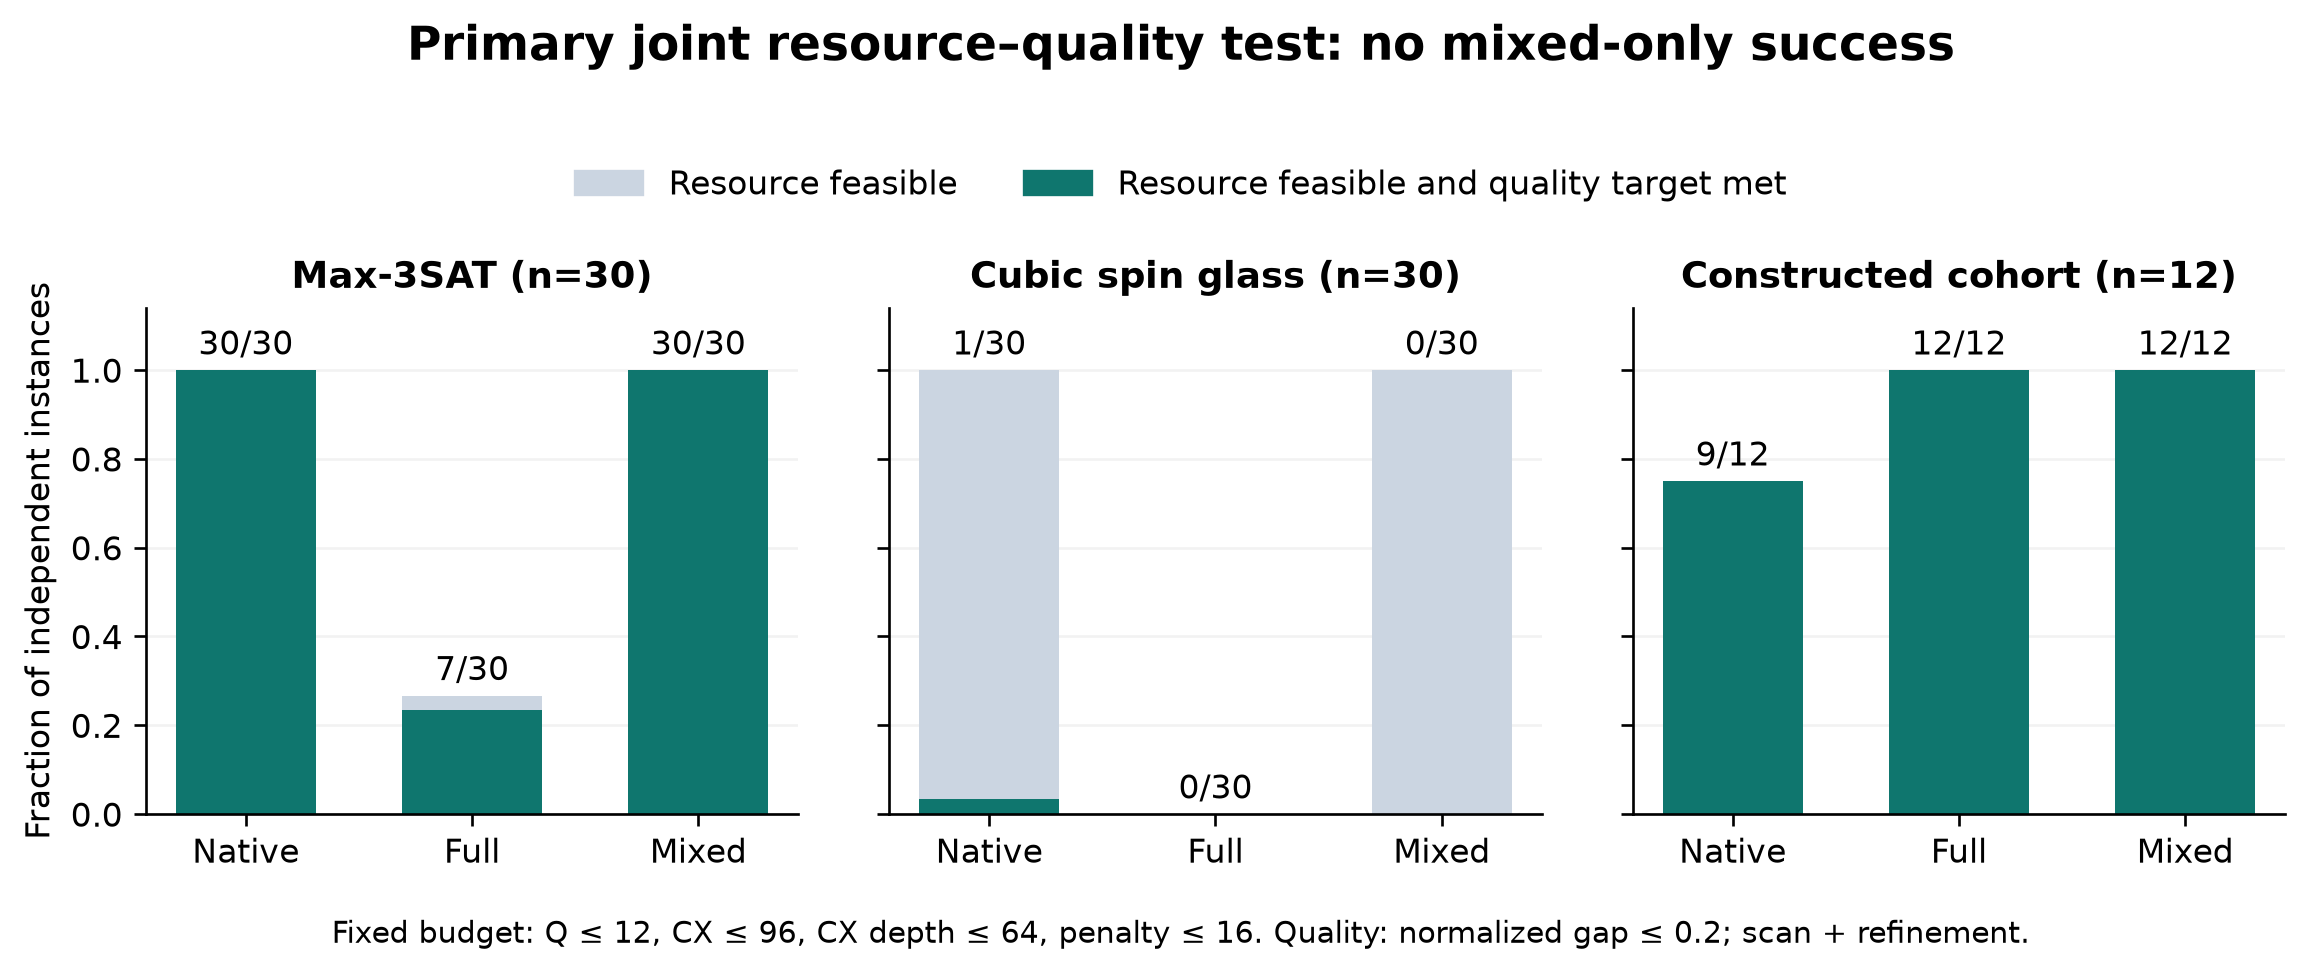
\includegraphics[width=\linewidth]{figures/primary_joint_results.png}
\caption{Primary joint-feasibility outcomes. Grey bars show resource
availability and green bars joint resource-and-quality success.}
\end{figure}

\subsection{Guardrail interventions and diagnostic prediction}
We compare no guardrail, a raw-moment guardrail, and a clipped prepared-state
guardrail on the same proper-mixed candidate library. Both diagnostics use
the declared design-independent normalisation and threshold $0.02$.
At device capacity alone, all three policies select identical actions on
all 72 instances. The rules are nevertheless not equivalent: among the
1,920 random-cohort mixed candidates, raw and prepared rules reject
1,243 and 1,329 candidates, with 86 eligibility disagreements. The lowest
resource-score candidate passes both rules in every case. Thus the observed
zero outcome difference reflects an inactive selection intervention, not
evidence that guardrails are generally effective or universally ineffective.
A degenerate zero bootstrap interval cannot establish a population-zero effect.

Separately, eight candidates per random instance were selected as diagnostic
probes before QAOA evaluation. On these 480 candidates from 60 instances,
leave-one-instance-out linear prediction controls auxiliary count, compiled
resource score, reduced-term count, prepared-state gap and family. Adding
the prepared diagnostic reduces held-out MSE for final auxiliary
inconsistency from $0.02862839$ to $0.02070590$. The instance-bootstrap
MSE improvement is $0.00792249$ with a descriptive 95\% interval
$[0.00376080,0.01273606]$. For final objective gap, MSE changes from
$0.00148790$ to $0.00139012$, with improvement interval
$[-0.00002862,0.00023108]$ including zero. Raw diagnostics show a similar
pattern. These secondary intervals are unadjusted and resample the computed
held-out instance errors without refitting all models in each bootstrap.
They provide limited predictive evidence for consistency in this model and
population, not causal selection benefit or reliable quality prediction.
The guardrail therefore remains an optional diagnostic.

\begin{figure}[htbp]\centering
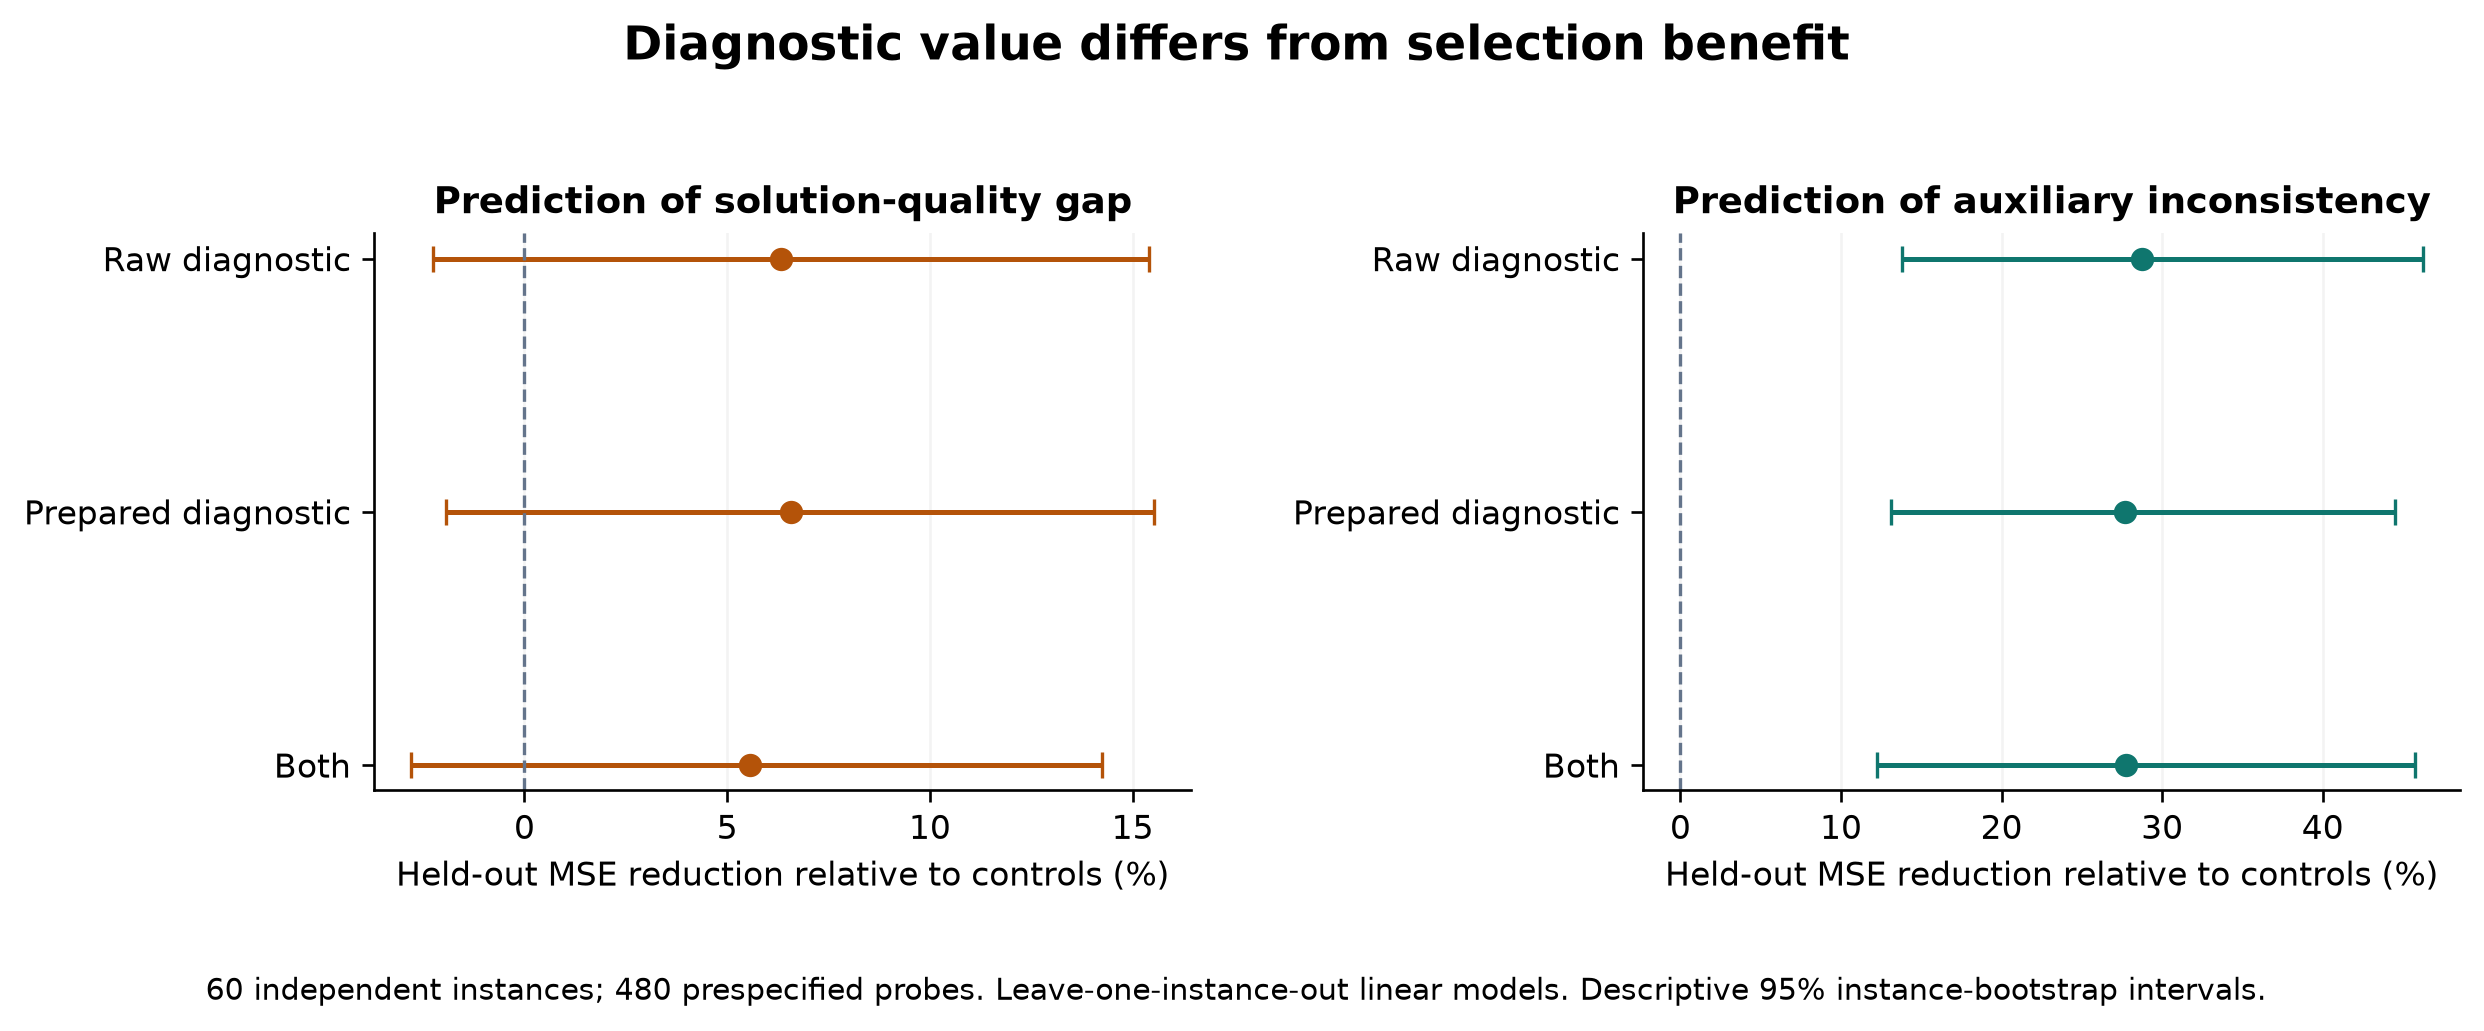
\includegraphics[width=\linewidth]{figures/diagnostic_prediction.png}
\caption{Relative held-out MSE improvement after adding diagnostics to the
control model. Bars are descriptive instance-bootstrap intervals.}
\end{figure}

\paragraph{Verification and scope.}
All 4,560 designs pass the pointwise and unique-lift checks.
Independent checks cover 9,120 product-law diagnostics, 1,086 saved
parameter sets, 1,350 grid points, 2,172 trace points, nine transpiled
statevector cases and six additionally recompiled explanatory witnesses.
The largest independent numerical difference is $1.57\times10^{-13}$.
Results are small-instance, noiseless and relative to one fixed compiler
configuration. The new protocol uses Nelder--Mead; it does not resolve the
previous cross-platform COBYLA trajectory discrepancy.
